\chapter{RESULTS}\label{resultsChapter}

This chapter summarizes our results, some of which were already discussed. The implementation of a flocking algorithm in OpenCL was covered in Section~\ref{flocksection} and the development of the RTPS modifier for the Blender Game Engine was detailed in Section~\ref{modifiersection}. 

This chapter presents benchmarks and demonstrations using the RTPS library and the RTPS modifier.

\section{Benchmarks}

%comments about the RTPS vs RTPS plot
We now provide timing results for our OpenCL implementation. We took benchmarks for both the RTPS standalone code (outside Blender) and the RTPS modifier. These timings were taken for a maximum number of particles set to 256K boids. The minimum distance was set to 1, with a searching radius of 1.5. Only the three main steering behaviors were considered in the benchmarks. The rules were equally weighted. The maximum allowable speed within the $10\times 10\times 10$ domain was 2. The boids were rendered as points in a simple scene with no other objects. The performance results of RTPS standalone and the RTPS modifier are shown in Figure~\ref{RTPSvsRTPS} with \textit{frames per second} (fps) as a function of the number of Boids in the scene. An acceptable frame rate for video games range between 30 fps and 60 fps. In general our GPU implementation runs at a frame rate that is over the acceptable range. 

% RTPS vs RTPS
\begin{figure}[htbp]
\begin{center}
\includegraphics[scale=0.7]{figures/RTPSvsRTPS.pdf}
\caption{Timings of RTPS-FLOCK system: FLOCK system from the standalone (outside the Blender Game Engine) and the FLOCK system from inside the Blender Game Engine.}
\label{RTPSvsRTPS}
\end{center}
\end{figure}

% comments about the RTPS vs Blender plot
We also compare the performance between our Boids system and the Blender's original Boids system with an identical number of Boids as well as with other parameters set to those in the previous experiment. Figure~\ref{RTPSvsBlender} shows the benchmark results. The RTPS-FLOCK system has better performance than the Blender-Boids system at all times, as expected from a GPU implementation. Our FLOCK system renders nearly 130K boids at frame rates above 30 fps. The Blender-Boids system can only render up to 8K boids at the acceptable fps range.

%RTPS vs Blender
\begin{figure}[htbp]
\begin{center}
\includegraphics[scale=0.7]{figures/benchmarks.pdf}
\caption{Timings of the RTPS modifier and the Blender-Boids system: the RTPS-GPU implementation outperforms the Blender-Boids system.}
\label{RTPSvsBlender}
\end{center}
\end{figure}

% comments about the speedup plot
The speedup of the RTPS-FLOCK system over the Blender-Boids system is seen in Figure~\ref{speedup}. The RTPS-FLOCK system is 20x faster than Blender-Boids system for flocks of 65K. The frame rate of Blender-Boids system for flocks with more than 65K boids is less than one frame per second.

% speedup 
\begin{figure}[htbp]
\begin{center}
\includegraphics[scale=0.7]{figures/speedup.pdf}
\caption{Speedup of the RTPS-FLOCK system compared to the original Blender-Boids system.}
\label{speedup}
\end{center}
\end{figure}

Comparing the performance of our implementation with some of the benchmarks that were mentioned in Section~\ref{flockingGPU}, our flocking implementation still has better performance. The library BehaveRT was used to run autonomous characters simulations in real-time. 
In this work Erra et al.\cite{BehaveRT} simulated 130K boids at 15 fps, compared to our results of 130K boids at 30 fps. The GPU computing device they used was a NVIDIA 8800GTS with 512 MB RAM while we used a NVIDIA 480GTX with 1.5 GB RAM. 

% comments about the timings per kernels
We also measured the performance of some of the kernels inside of the RTPS-FLOCK system. The parameter's settings were the same as for the previous tests. The searching radius was constant throughout the benchmarks. Figure~\ref{kernelBench} shows that most of the kernels took the same amount of time for the different flock sizes. The only kernel that increased the time spent to be computed was the Rules kernel. This increase in time results from maintaining a fixed searching radius, which leads to an increasing number of neighboring boids. If the searching radius doubles, the average number of neighbors increases by 4x in 2D and 8x in 3D, given a constant average separation between boids. 

% benchmarks per kernels 
\begin{figure}[htbp]
\begin{center}
\includegraphics[scale=0.7]{figures/kernelsPlot.pdf}
\caption{Kernels timings of the RTPS-FLOCK system.}
\label{kernelBench}
\end{center}
\end{figure}


% demos
\section{Demos}

\subsection{Symmetry Demo}
As discussed previously, the three main rules of flocking are: 1) \textit{separation}, 2) \textit{alignment}, and 3) \textit{cohesion}. The velocity of each boid is the result of a linear combination of three effects, each one with its own scalar weight parameter. We seek to better understand the effect of each of these parameters. Consider first each effect taken in isolation.

The property of each term is best visualized with an initial configuration of boids that is symmetric, which also helps when debugging the code. To this end, we uniformly space the boids in a rectangular configuration.  From symmetry arguments, a boid in the top-left quadrant has the same relationship with respect to its neighbors as a boid in the same relative location in each of the other three quadrants. Thus the four-fold symmetry of the rectangle will be maintained during the time evolution of the boids. Figure~\ref{alignRule} shows the starting conditions of the boids. The symmetric motion that results from the \textit{separation} and \textit{cohesion} rules are shown in Figures~\ref{sepRule} and~\ref{cohRule}, respectively. These figures show 144 boids in a centralized square inside a $5\times 5\times 5$ grid.

The case of alignment is somewhat different since it is the boid velocities that must be taken into consideration. If the initial boid velocities are not symmetric, geometric symmetry is not maintained. 

% alignment
\begin{figure}[htbp]
\begin{center}
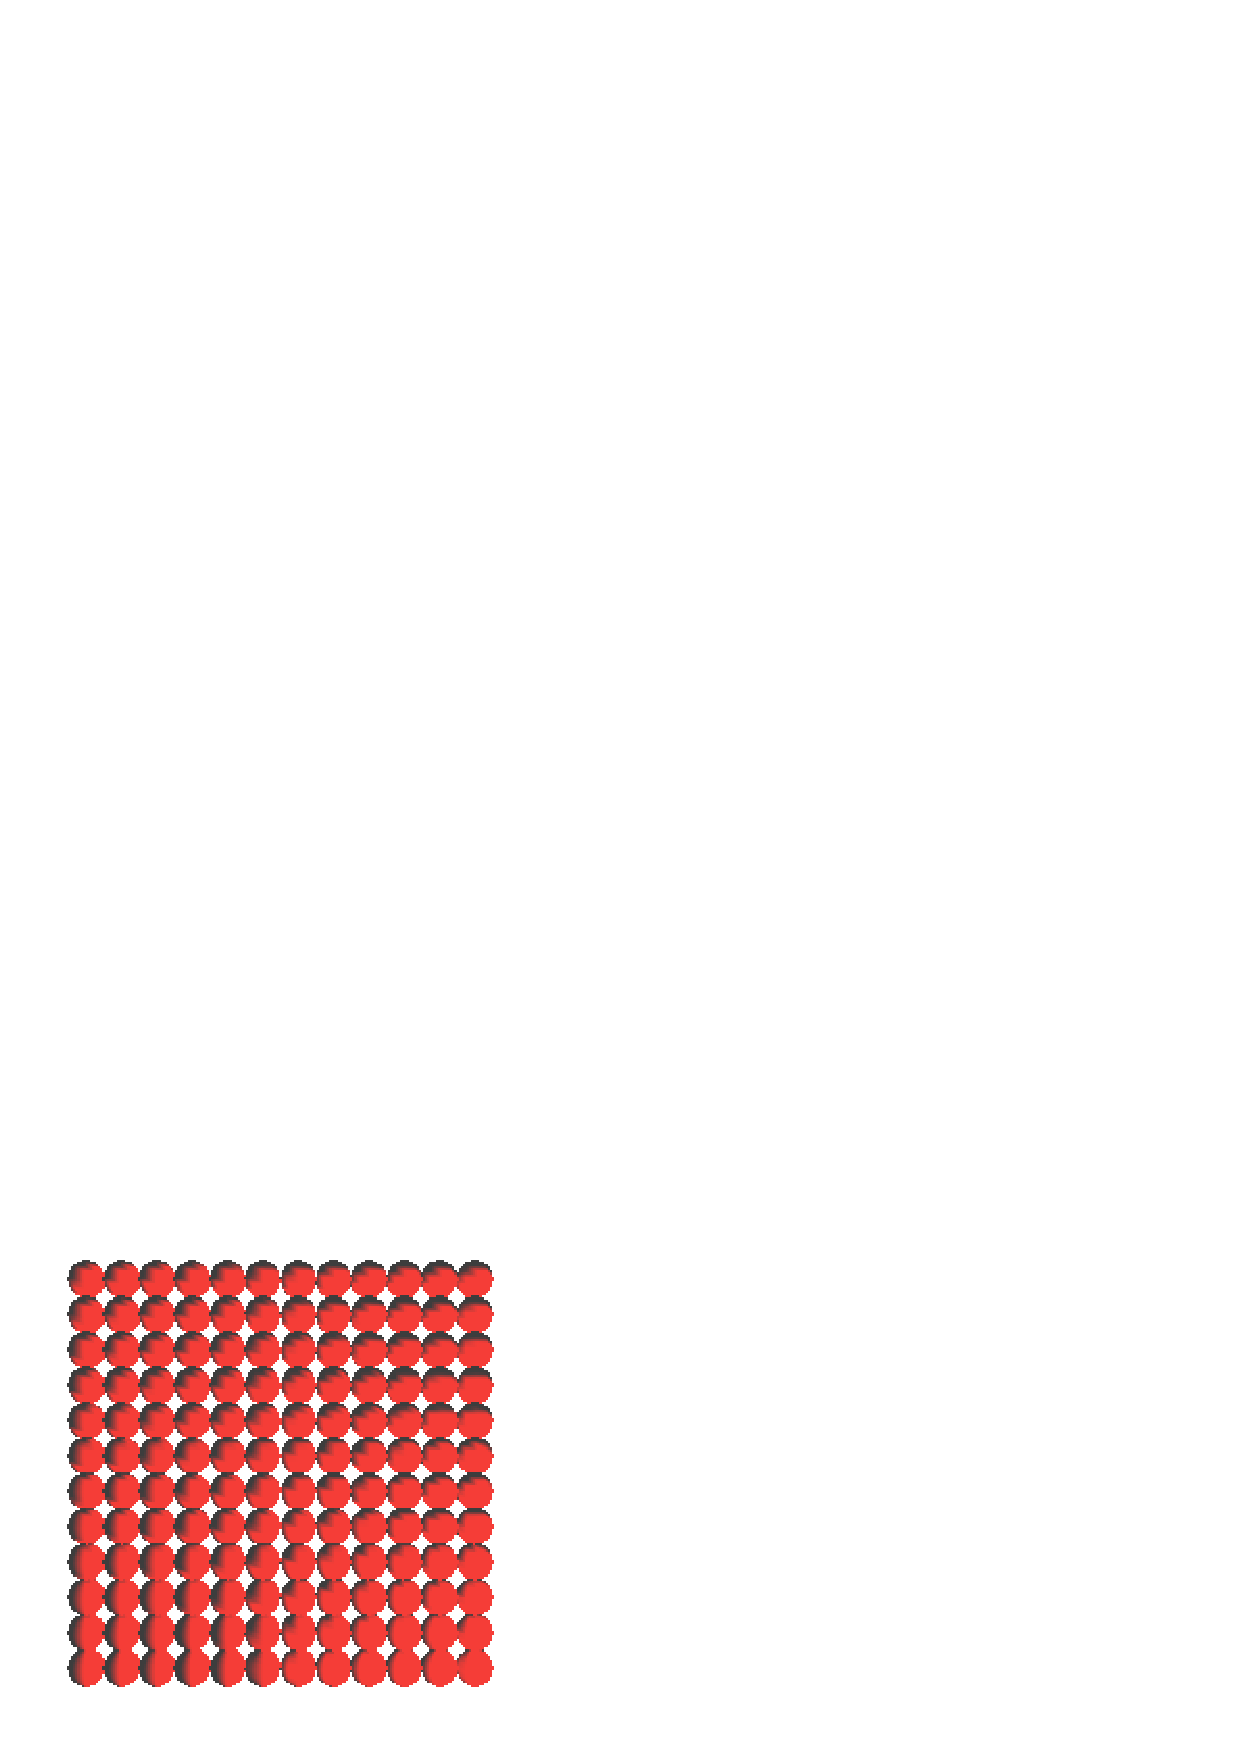
\includegraphics[scale=0.5]{figures/align.pdf}
\caption{Initial boid state: the scalar weights for each of the rules are zero; the boids are equally spaced, forming a square.}
\label{alignRule}
\end{center}
\end{figure}

% separation
\begin{figure}[htbp]
\begin{center}$
\begin{array}{cc}
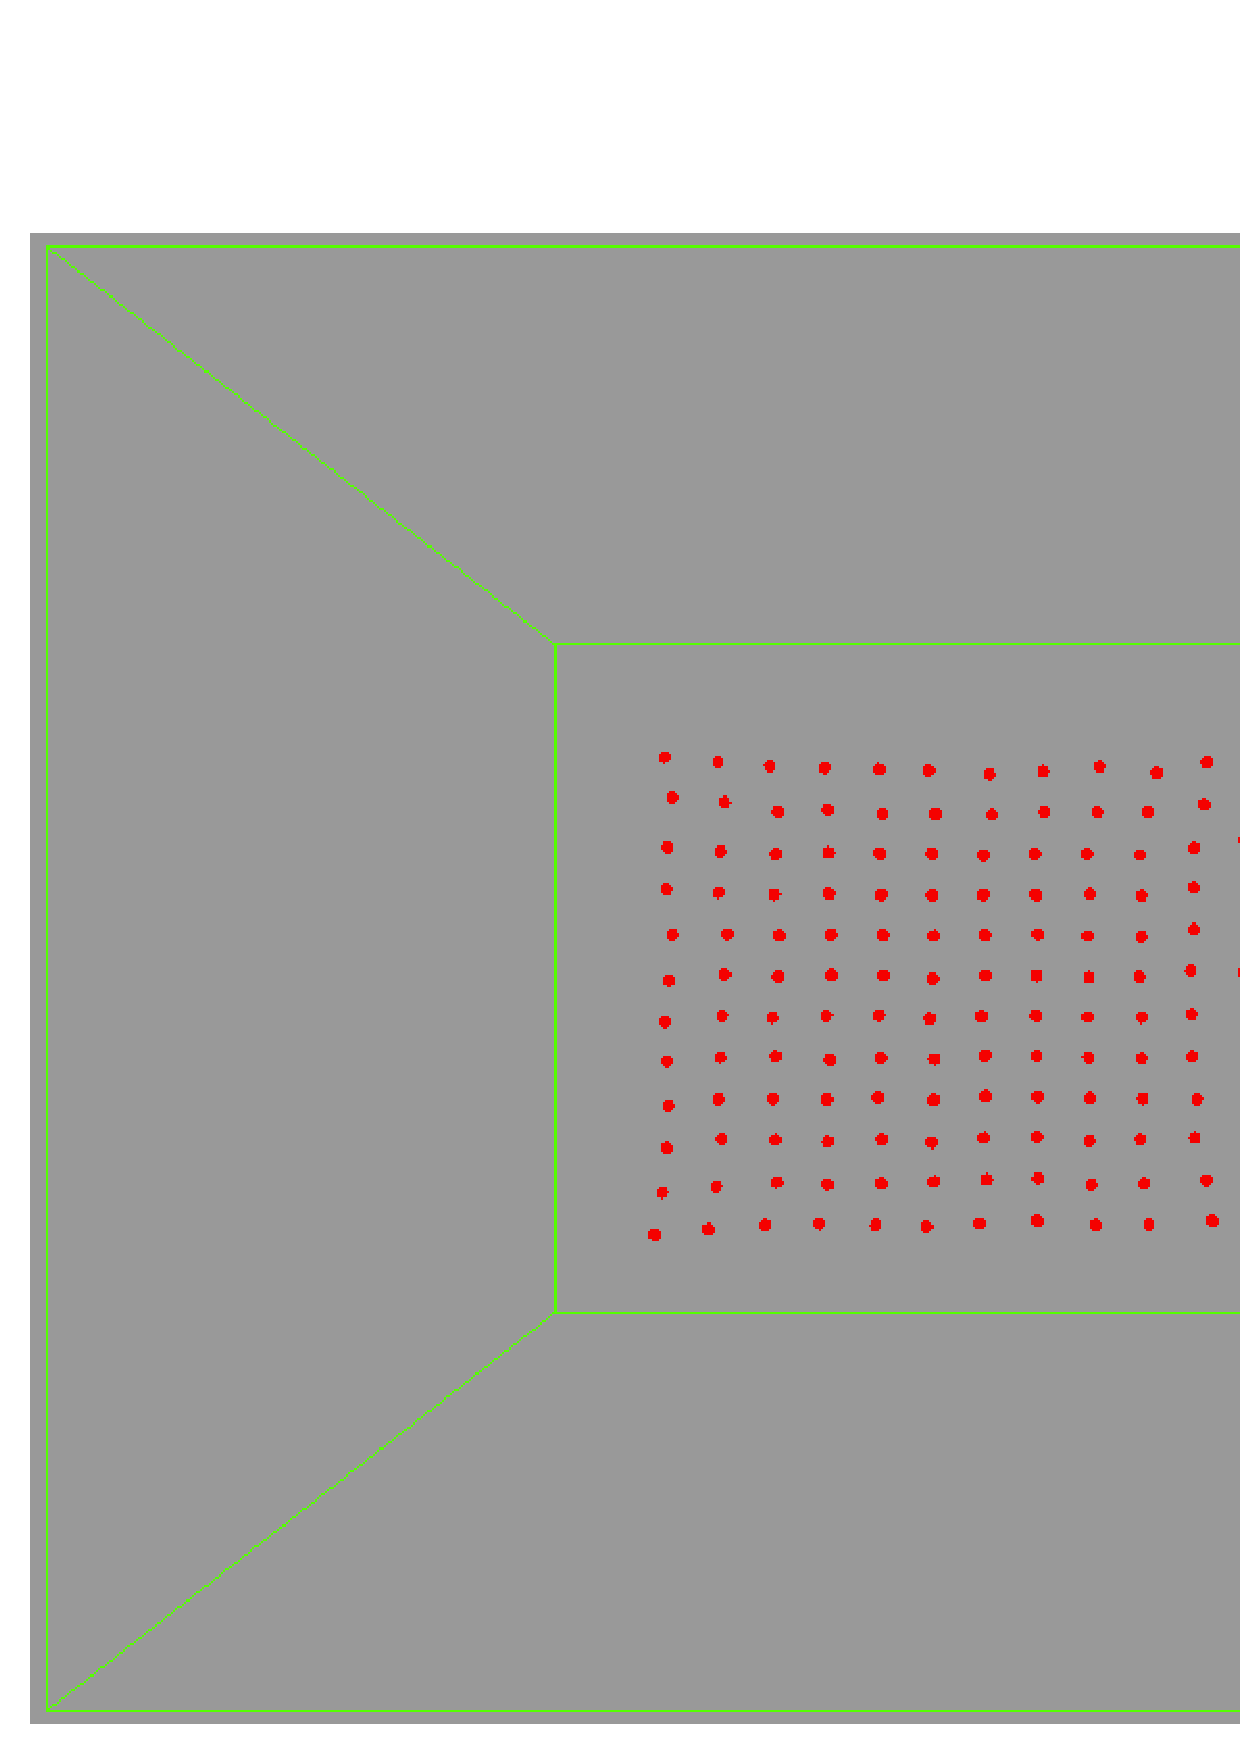
\includegraphics[scale= 0.5]{figures/sep1.pdf} &
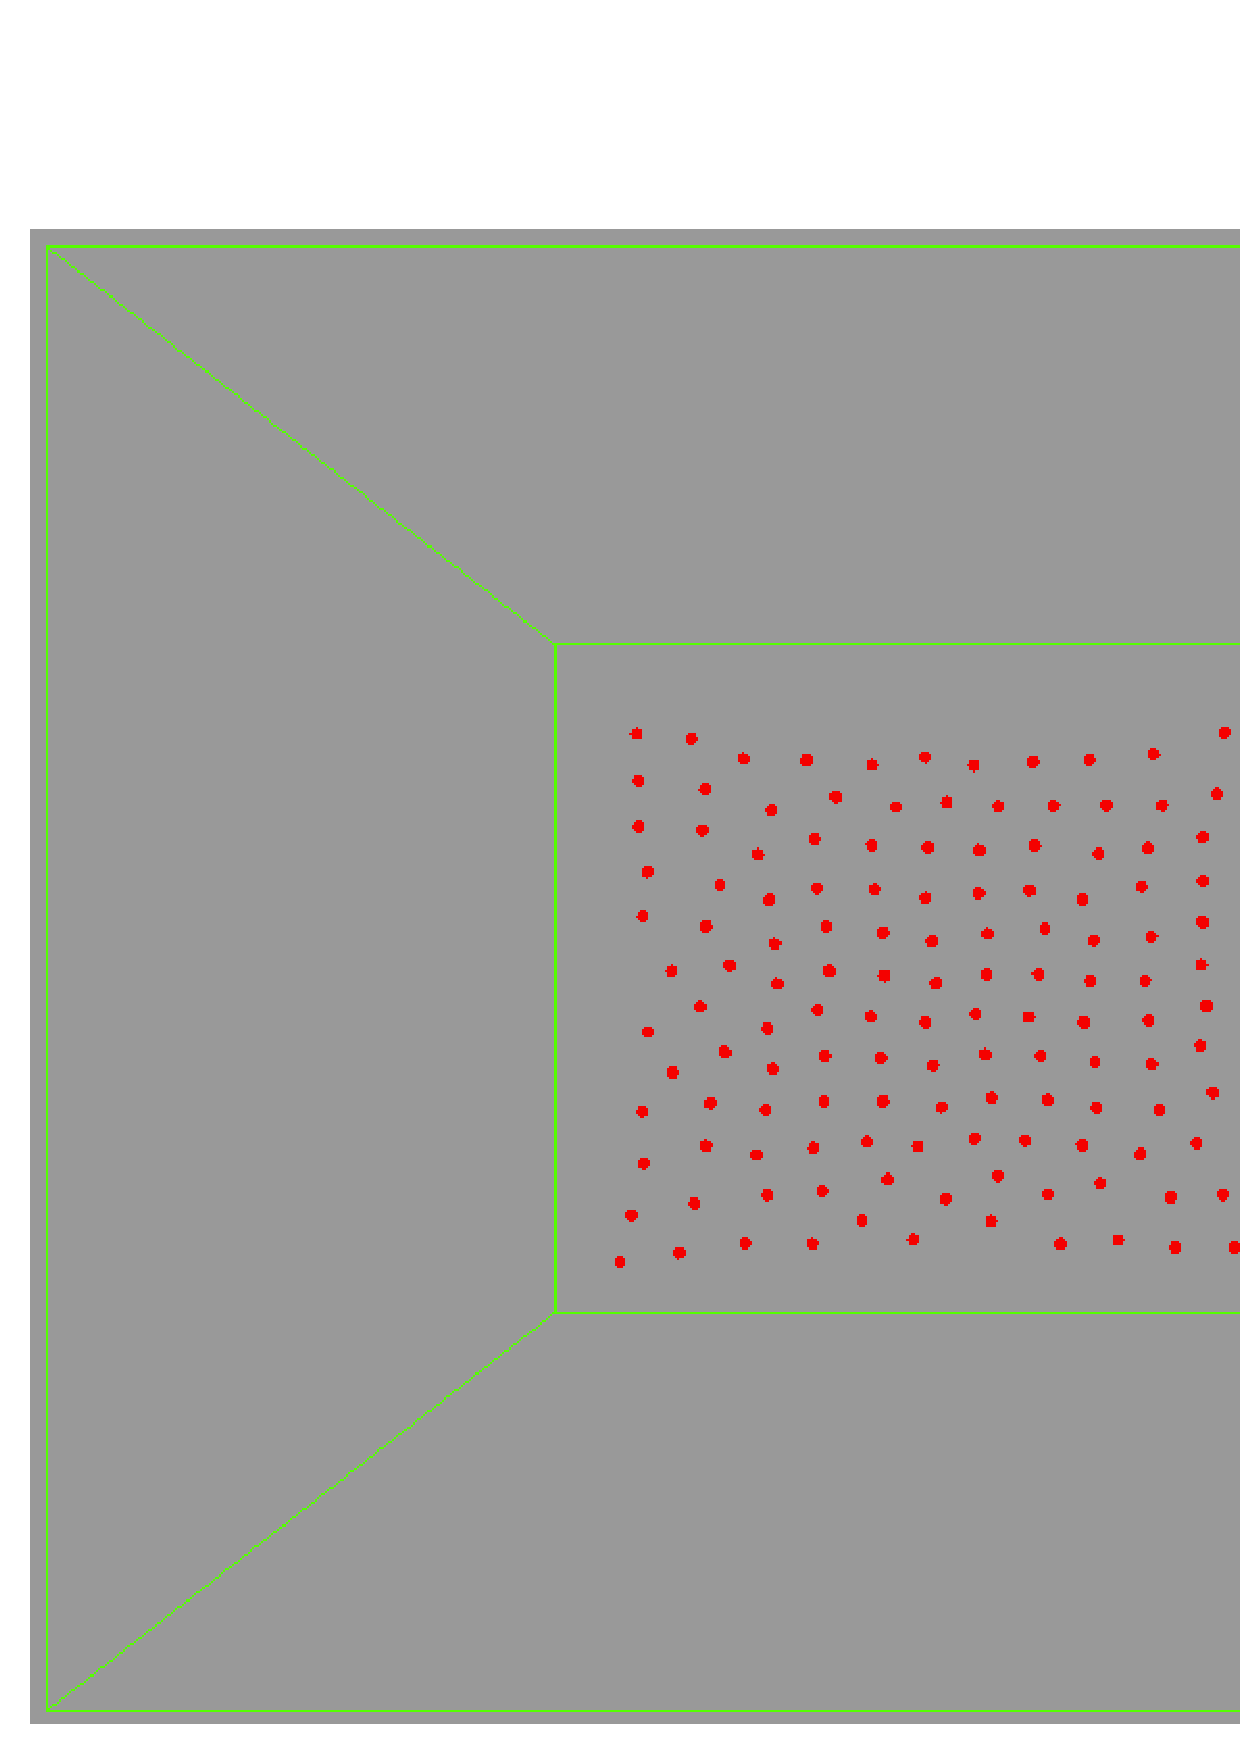
\includegraphics[scale= 0.5]{figures/sep2.pdf}
\end{array}$
\end{center}
\caption{Screenshots of the symmetry of the \textit{separation} rule: the weight for \textit{separation} is set to 1 while the weights of the other rules are set to zero, the maximum speed and searching radius are 2, and the minimum separation distance is 1.5. The boids spread out symmetrically.}
\label{sepRule}
\end{figure}

% cohesion
\begin{figure}[htbp]
\begin{center}
\begin{tabular}{cc}
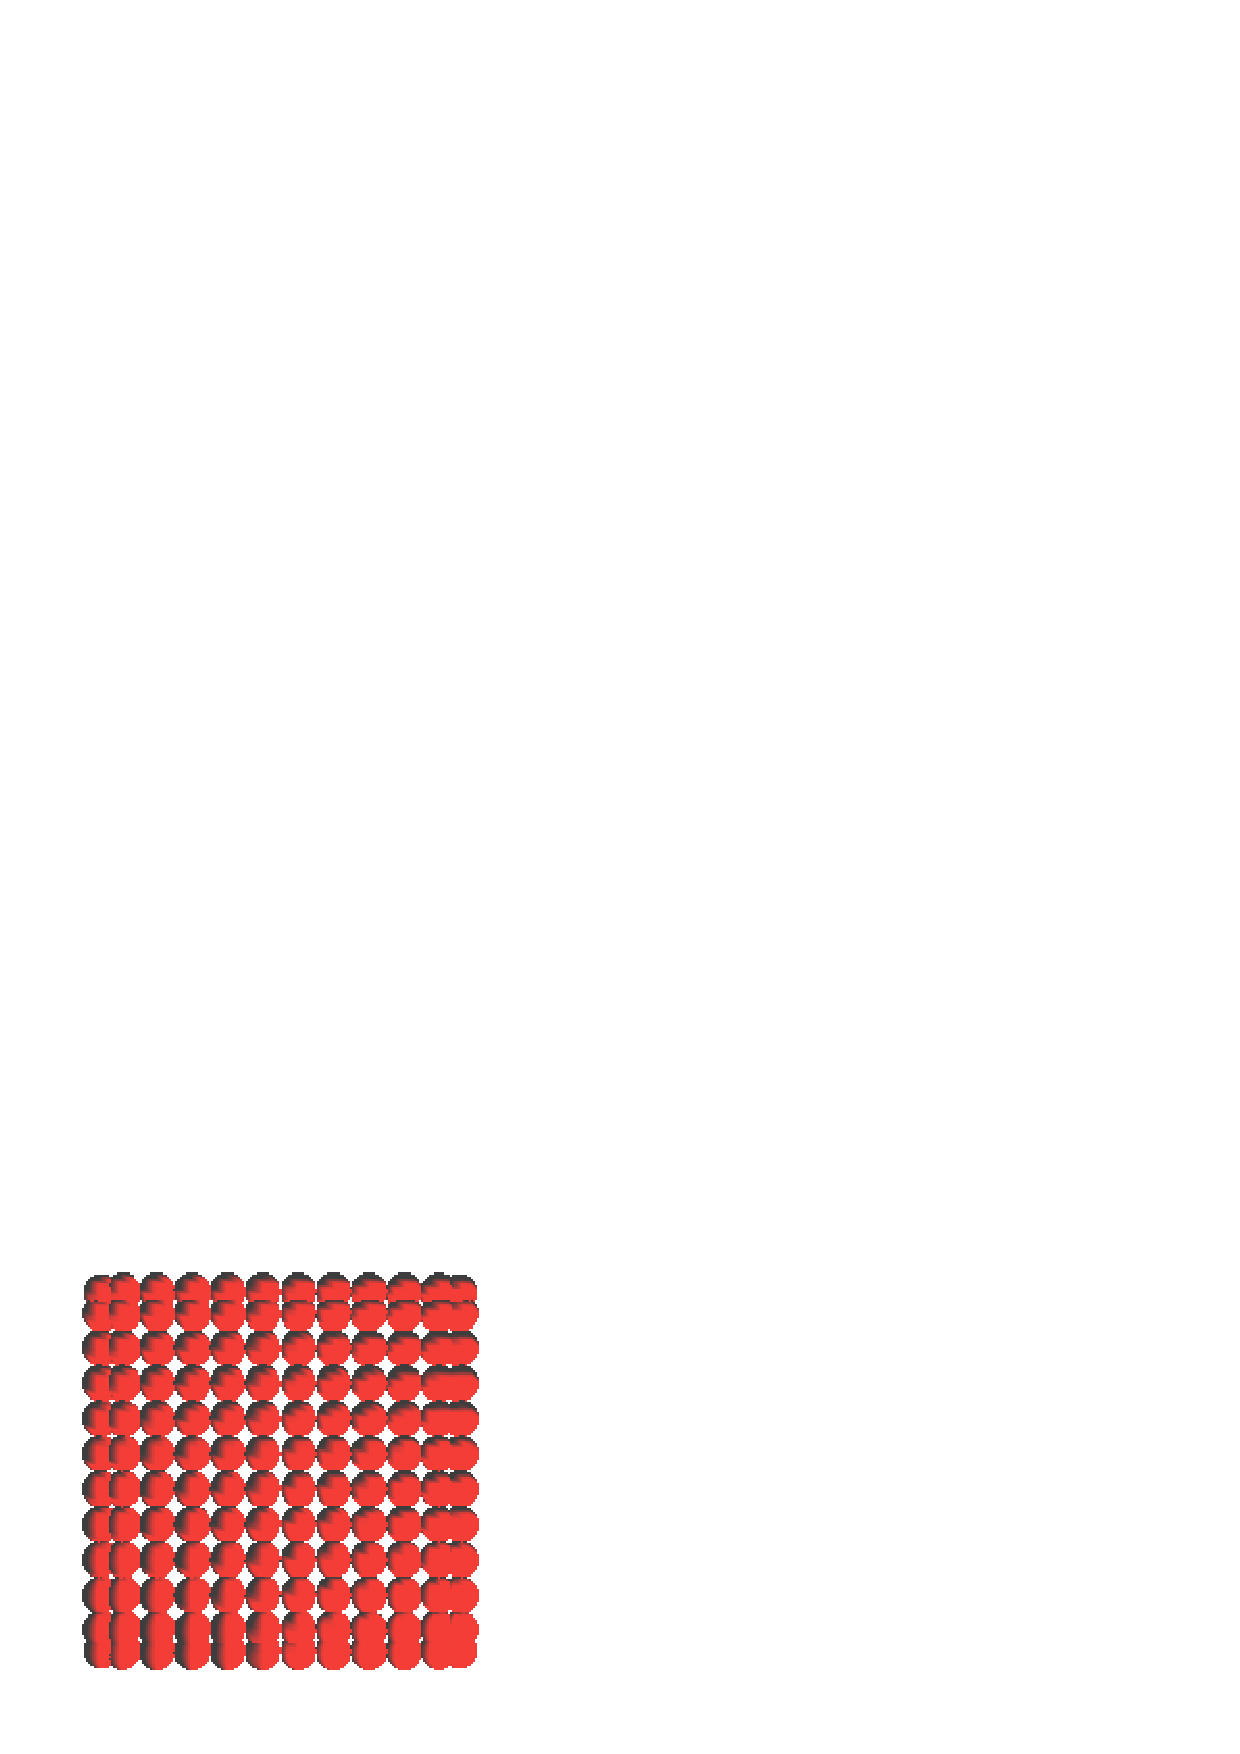
\includegraphics[scale= 0.5]{figures/coh1.pdf} &
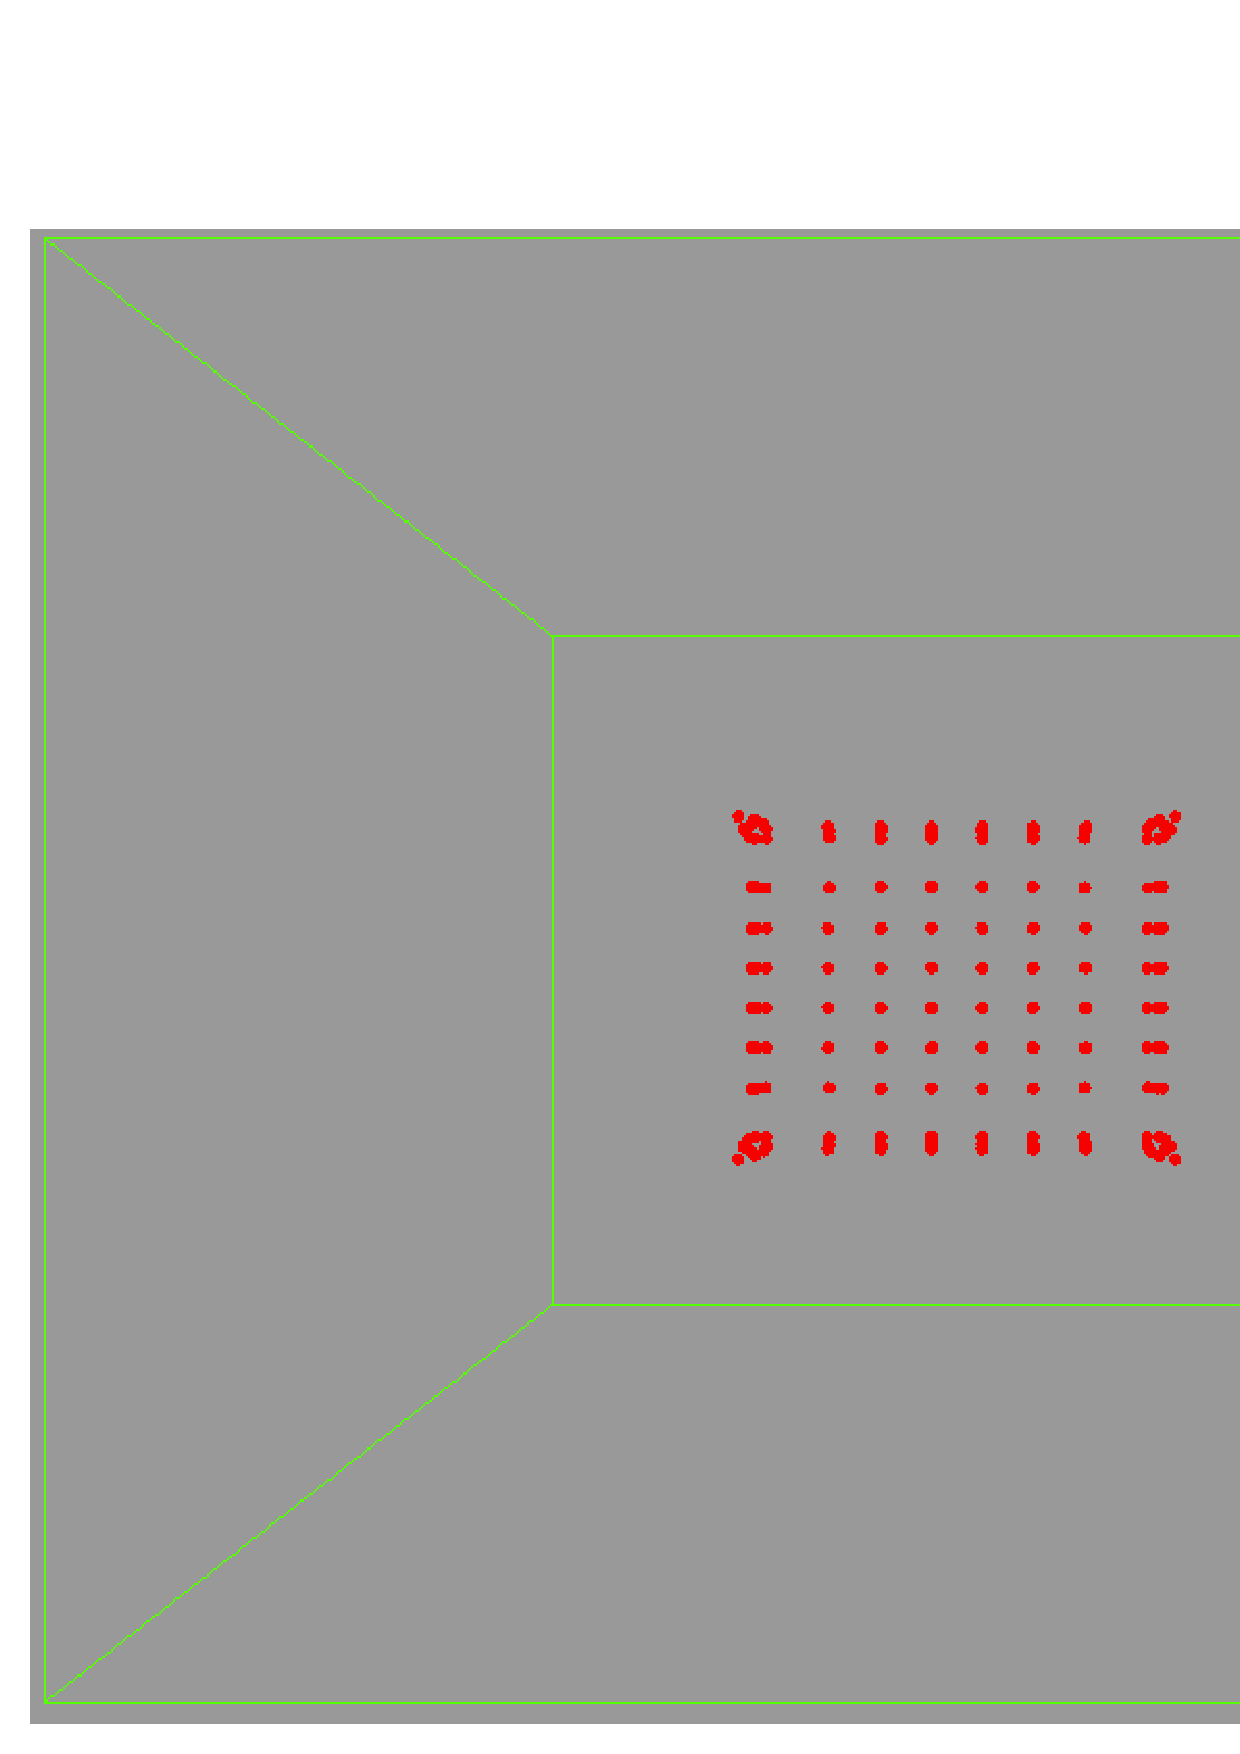
\includegraphics[scale= 0.5]{figures/coh2.pdf} \\
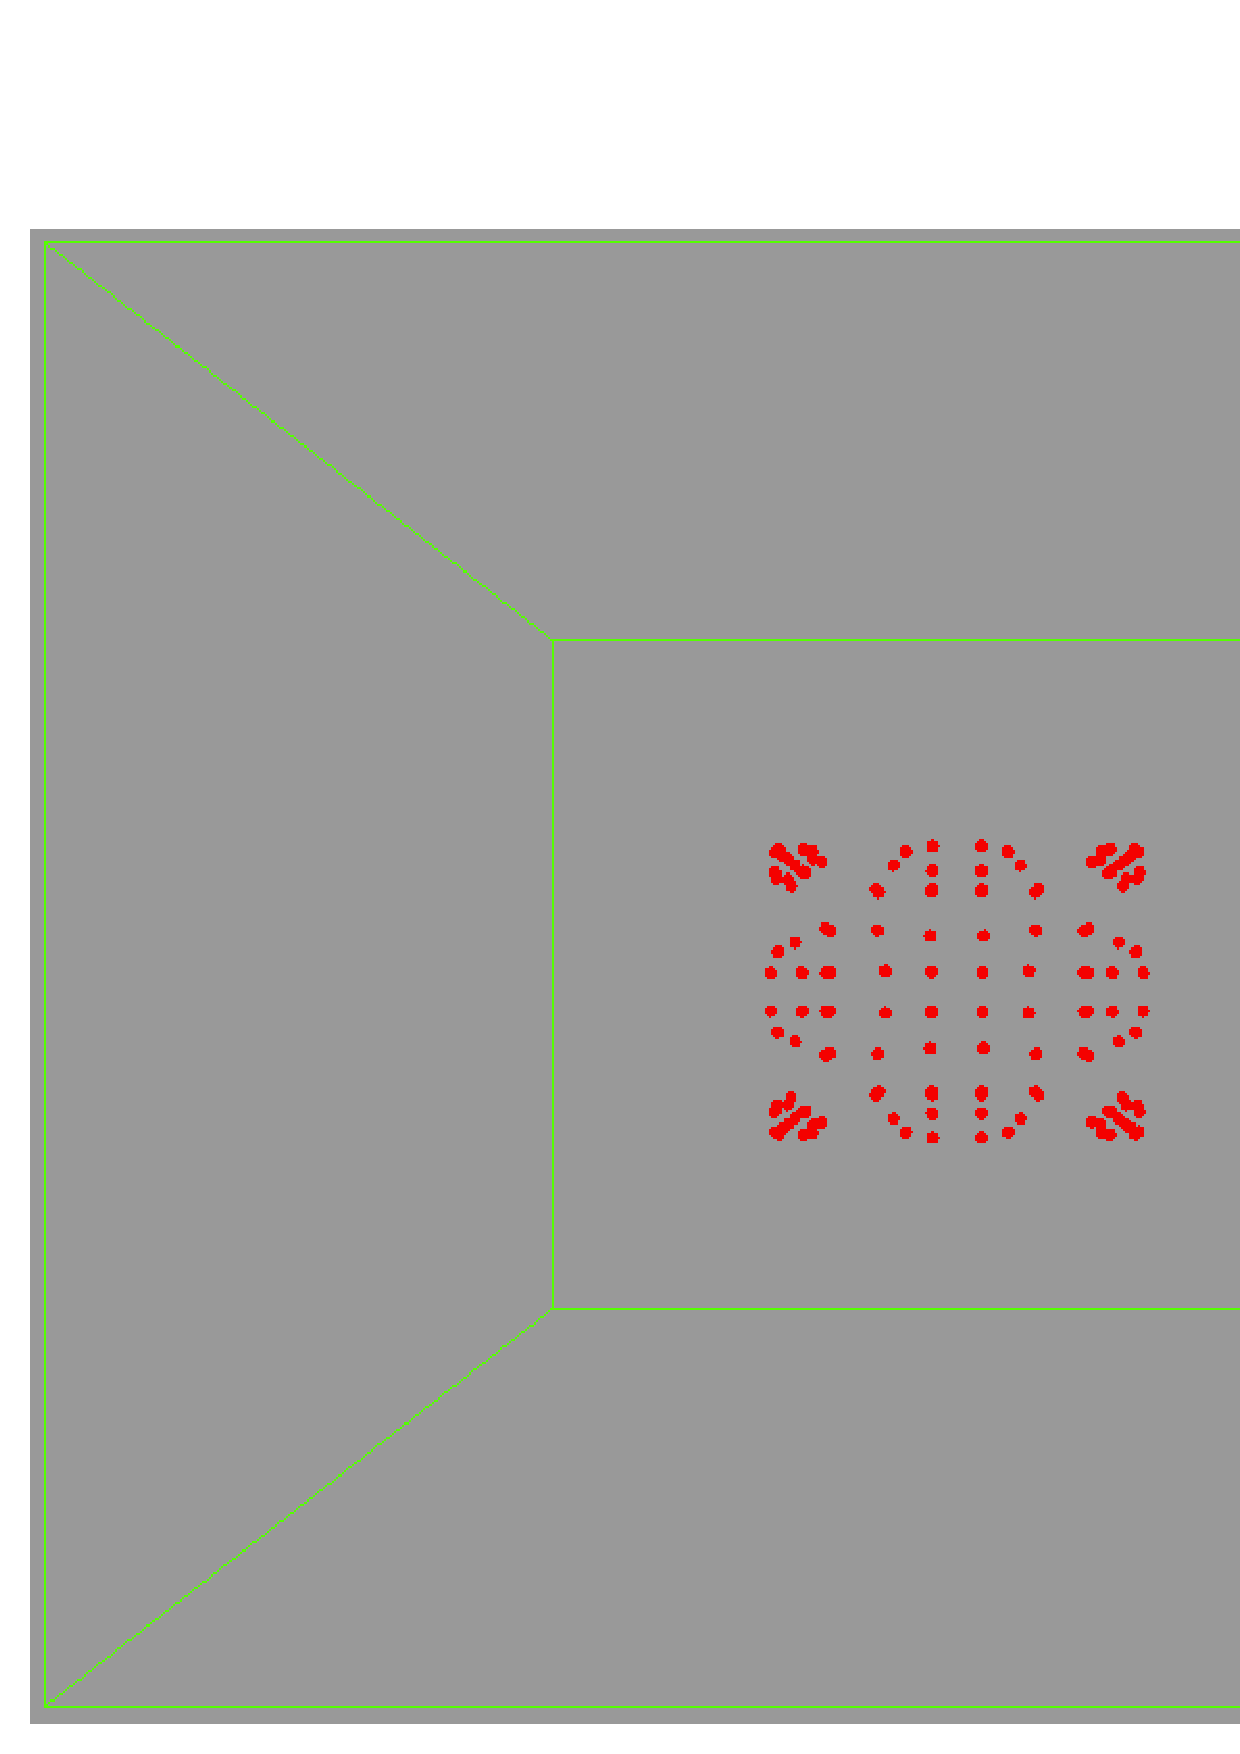
\includegraphics[scale= 0.5]{figures/coh3.pdf} &
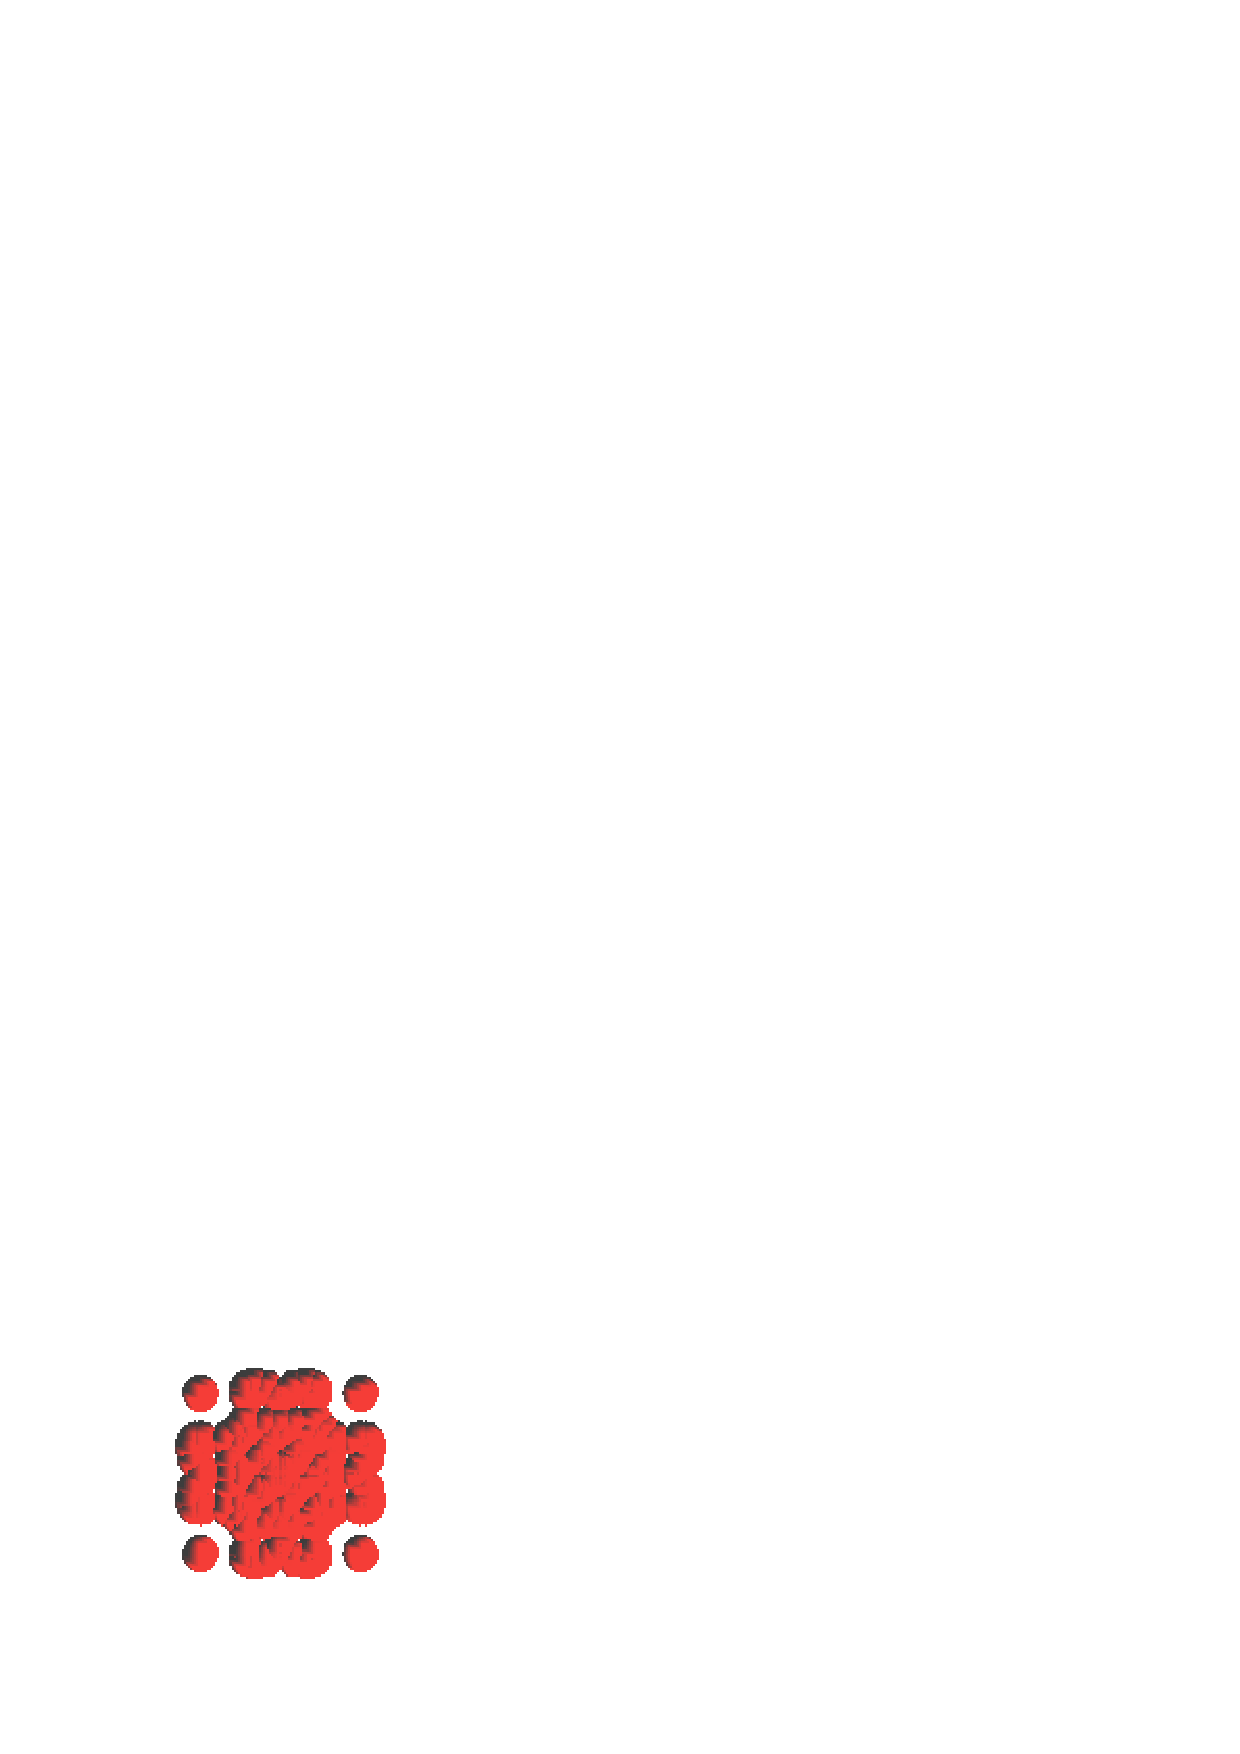
\includegraphics[scale= 0.5]{figures/coh4.pdf}
\end{tabular}
\end{center}
\caption{Screenshots of the symmetry of the \textit{cohesion} rule: the scalar weight for the \textit{cohesion} rule is set to 1 while the weights for the other rules are set to zero, the maximum speed is 2, and the searching radius is 1. The boids move towards the center causing the flock to form symmetric shapes.}
\label{cohRule}
\end{figure}

% Goal demo
\subsection{Goal Demo}
The \textit{goal}, \textit{avoid}, and \textit{following the leader} rules can only be used in the RTPS standalone code. They have not yet been added to the RTPS modifier for use inside the Blender Game Engine. 

In the next demo, we simulate a ``\textit{swarm of bees}''. The bees try to approach their target (a blue box) which represents their hive. The center of the box is used as the coordinates of the target. In this demo, 648 boids were simulated. Only the \textit{goal} and \textit{separation} rules are taken into consideration. The scalar weights for \textit{goal} and \textit{separation} are 1 and 0.5, respectively. The maximum speed is set to 2, with a searching radius of 1.5. 

\begin{figure}[htbp]
\begin{center}$
\begin{array}{ccc}
\includegraphics[scale=0.35]{figures/demo_goal1.pdf} &&
\includegraphics[scale=0.35]{figures/demo_goal2.pdf} \\ \\
\includegraphics[scale=0.35]{figures/demo_goal3.pdf} &&
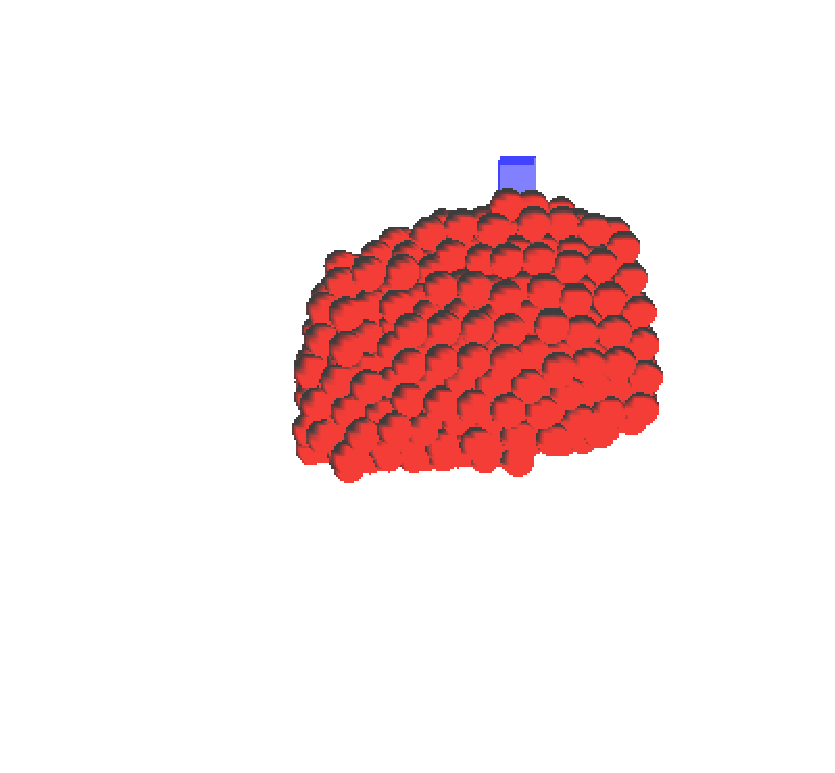
\includegraphics[scale=0.35]{figures/demo_goal4.pdf} \\ \\
\includegraphics[scale=0.35]{figures/demo_goal5.pdf} &&
\includegraphics[scale=0.35]{figures/demo_goal6.pdf}
\end{array}$
\end{center}
\caption{Screenshots of the ``\textit{swarm of bees}'' simulation: there are 648 boids and the blue cube is the target of the flock.}
\label{demo_goal}
\vspace{16pt}
\end{figure}
 
Figure~\ref{demo_goal} shows a series of screenshots of bee flocking. The flock starts from an artificial shape of a cube. The boids start to approach the target until they reach it. Once the boids find the target, they remain in the target neighborhood. 

We ran another demo in which the three main steering behaviors, together with the \textit{goal} rule were used to compute the behavior of the boids. Figure~\ref{goal_4rules} shows the resulting flock. Each rule was weighted equally. A minimum separation distance of 2 and a searching radius of 2.5 were used. The initial positions of the boids were identical to the conditions in Figure~\ref{demo_goal}. From the Figure we see that the boids are more separated than in the first example. This is because we are using the \textit{separation} rule with a minimum separation distance that is double the initial distance that separates the boids. Although all four rules were taken into account, we see that the overall flock objective (reach the target) was achieved. 

% 4 rules
\begin{figure}[htbp]
\begin{center}
\includegraphics[scale=0.35]{figures/demo_goal_4rules.pdf}
\caption{Screenshot of the flock when it reached its the target: \textit{separation}, \textit{alignment}, \textit{cohesion}, and \textit{goal} rules were used to compute the behavior of the boids.}
\label{goal_4rules}
\end{center}
\end{figure}

% Blender demo
\subsection{Blender Demo}

The following Blender demo of the RTPS library uses one hose that emits 500 boids. This demo simulates a ``\textit{crowd of people}'', whose motion is two-dimensional. Figure~\ref{crowd_prop} shows the properties used to create the hose, and Figure~\ref{crowd_modifier} shows the parameter settings. 

\begin{figure}[htbp]
\begin{center}
\includegraphics[scale=0.7]{figures/demo_crowds_prop.pdf}
\caption{Logic Editor properties area showing the properties used to create the hose of the ``\textit{crowding}'' simulation demo.}
\label{crowd_prop}
\end{center}
\end{figure}

\begin{figure}[htbp]
\begin{center}
\includegraphics[scale=0.8]{figures/demo_crowds_modifier.pdf}
\caption{RTPS modifier showing the settings of the ``\textit{crowding}'' simulation demo.}
\label{crowd_modifier}
\end{center}
\end{figure}

Figure~\ref{crowd_shots} shows the screenshots of the demo. The emitter hose starts emitting the boids at the center of the world (physical domain of the system). The boids start to react according to the settings of the simulation. Finally, the boids are spread out into the world domain while still following the rules.

\begin{figure}[htbp]
\begin{center}$
\begin{array}{c}
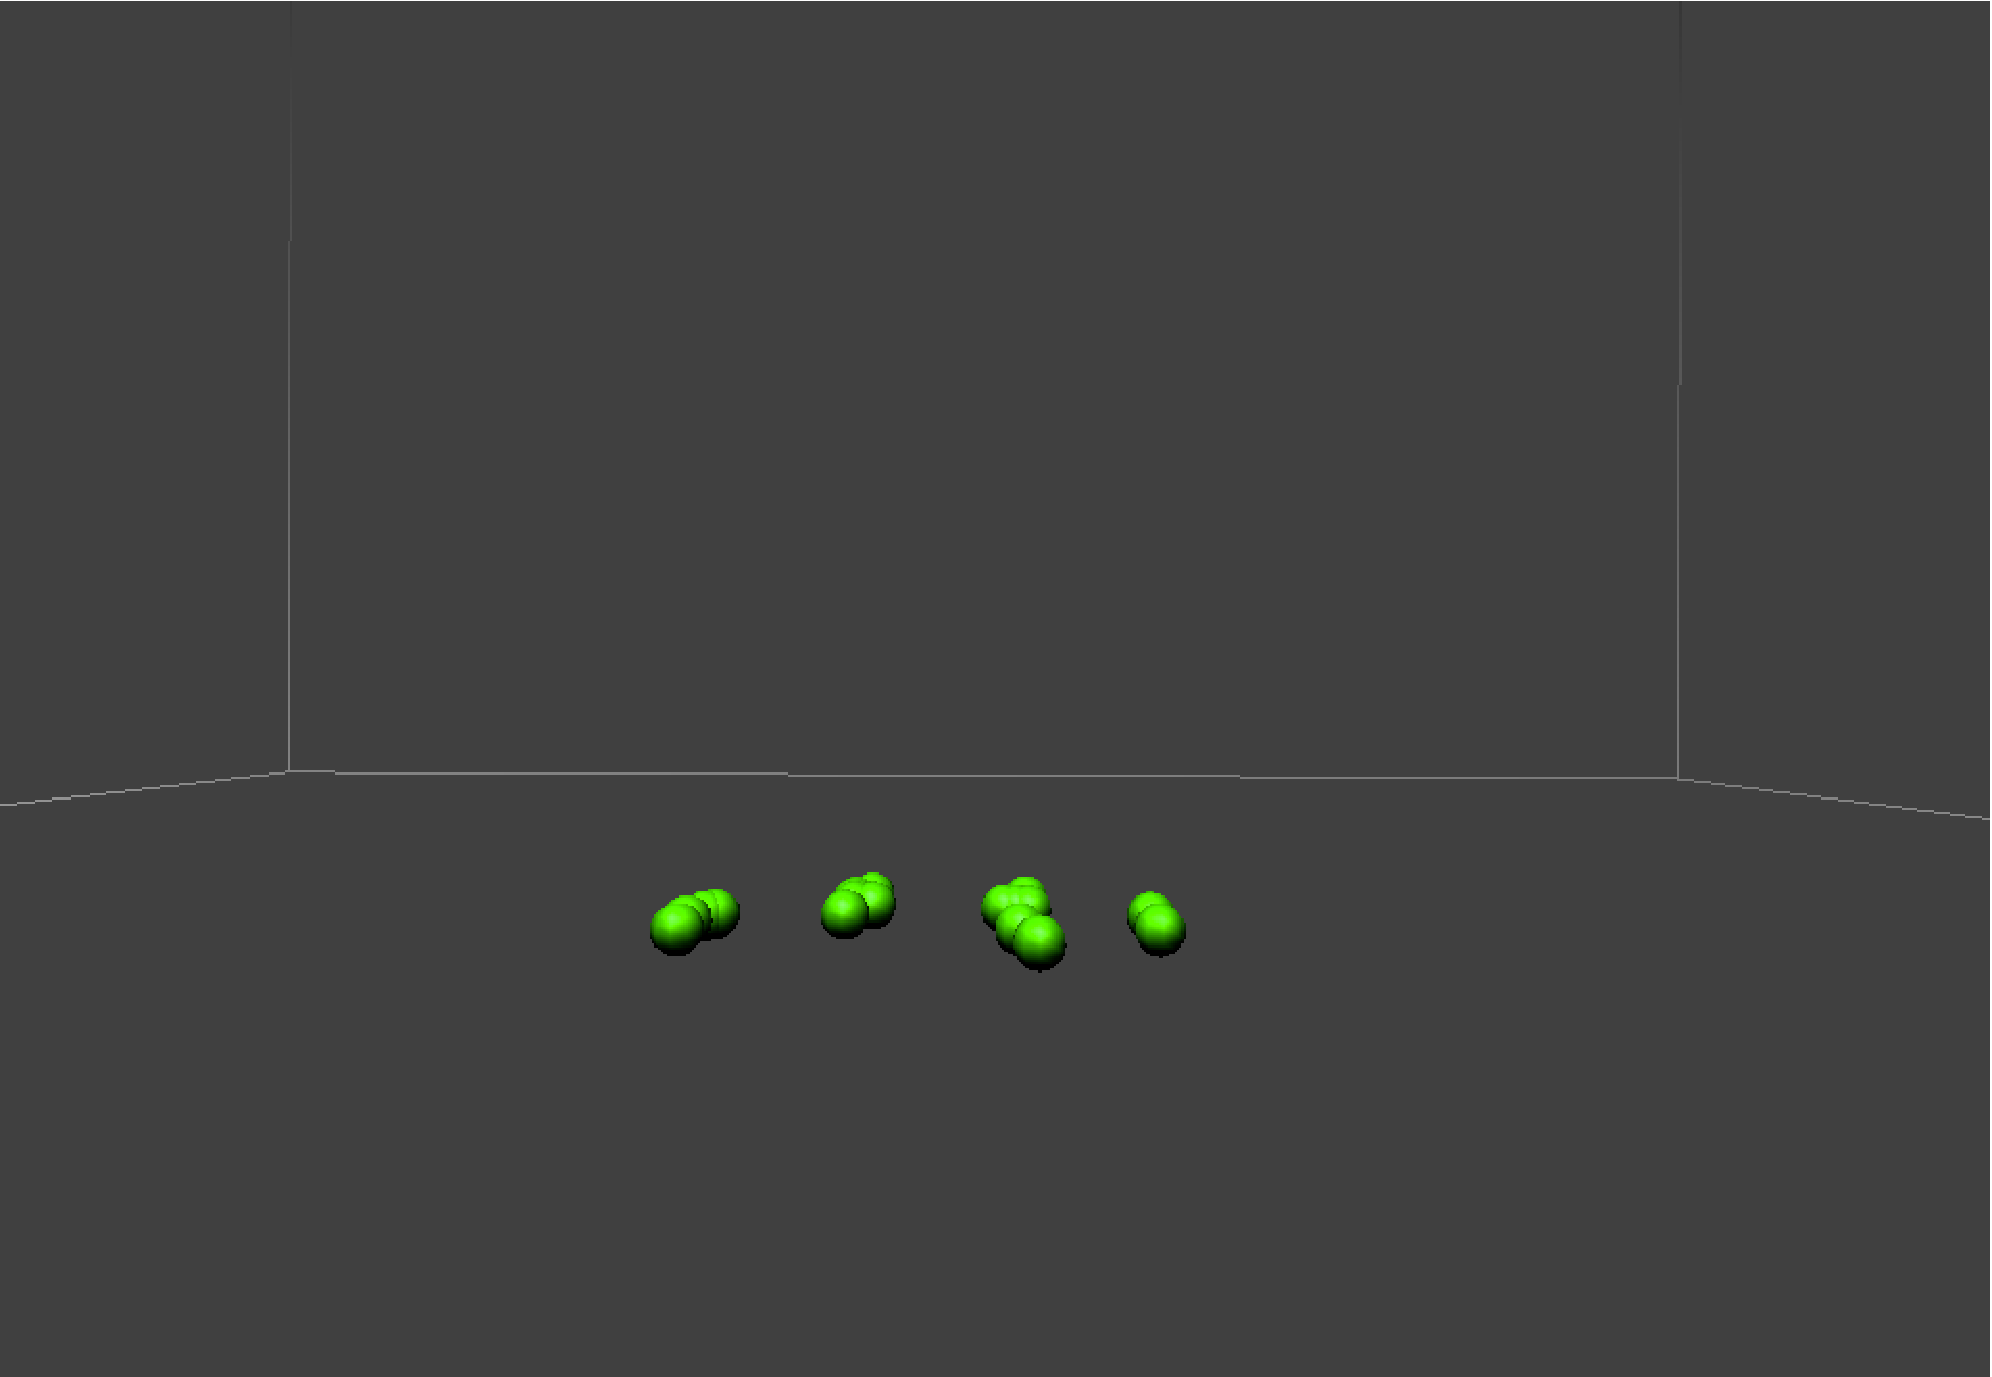
\includegraphics[scale=0.28]{figures/demo_crowds1.pdf} \\
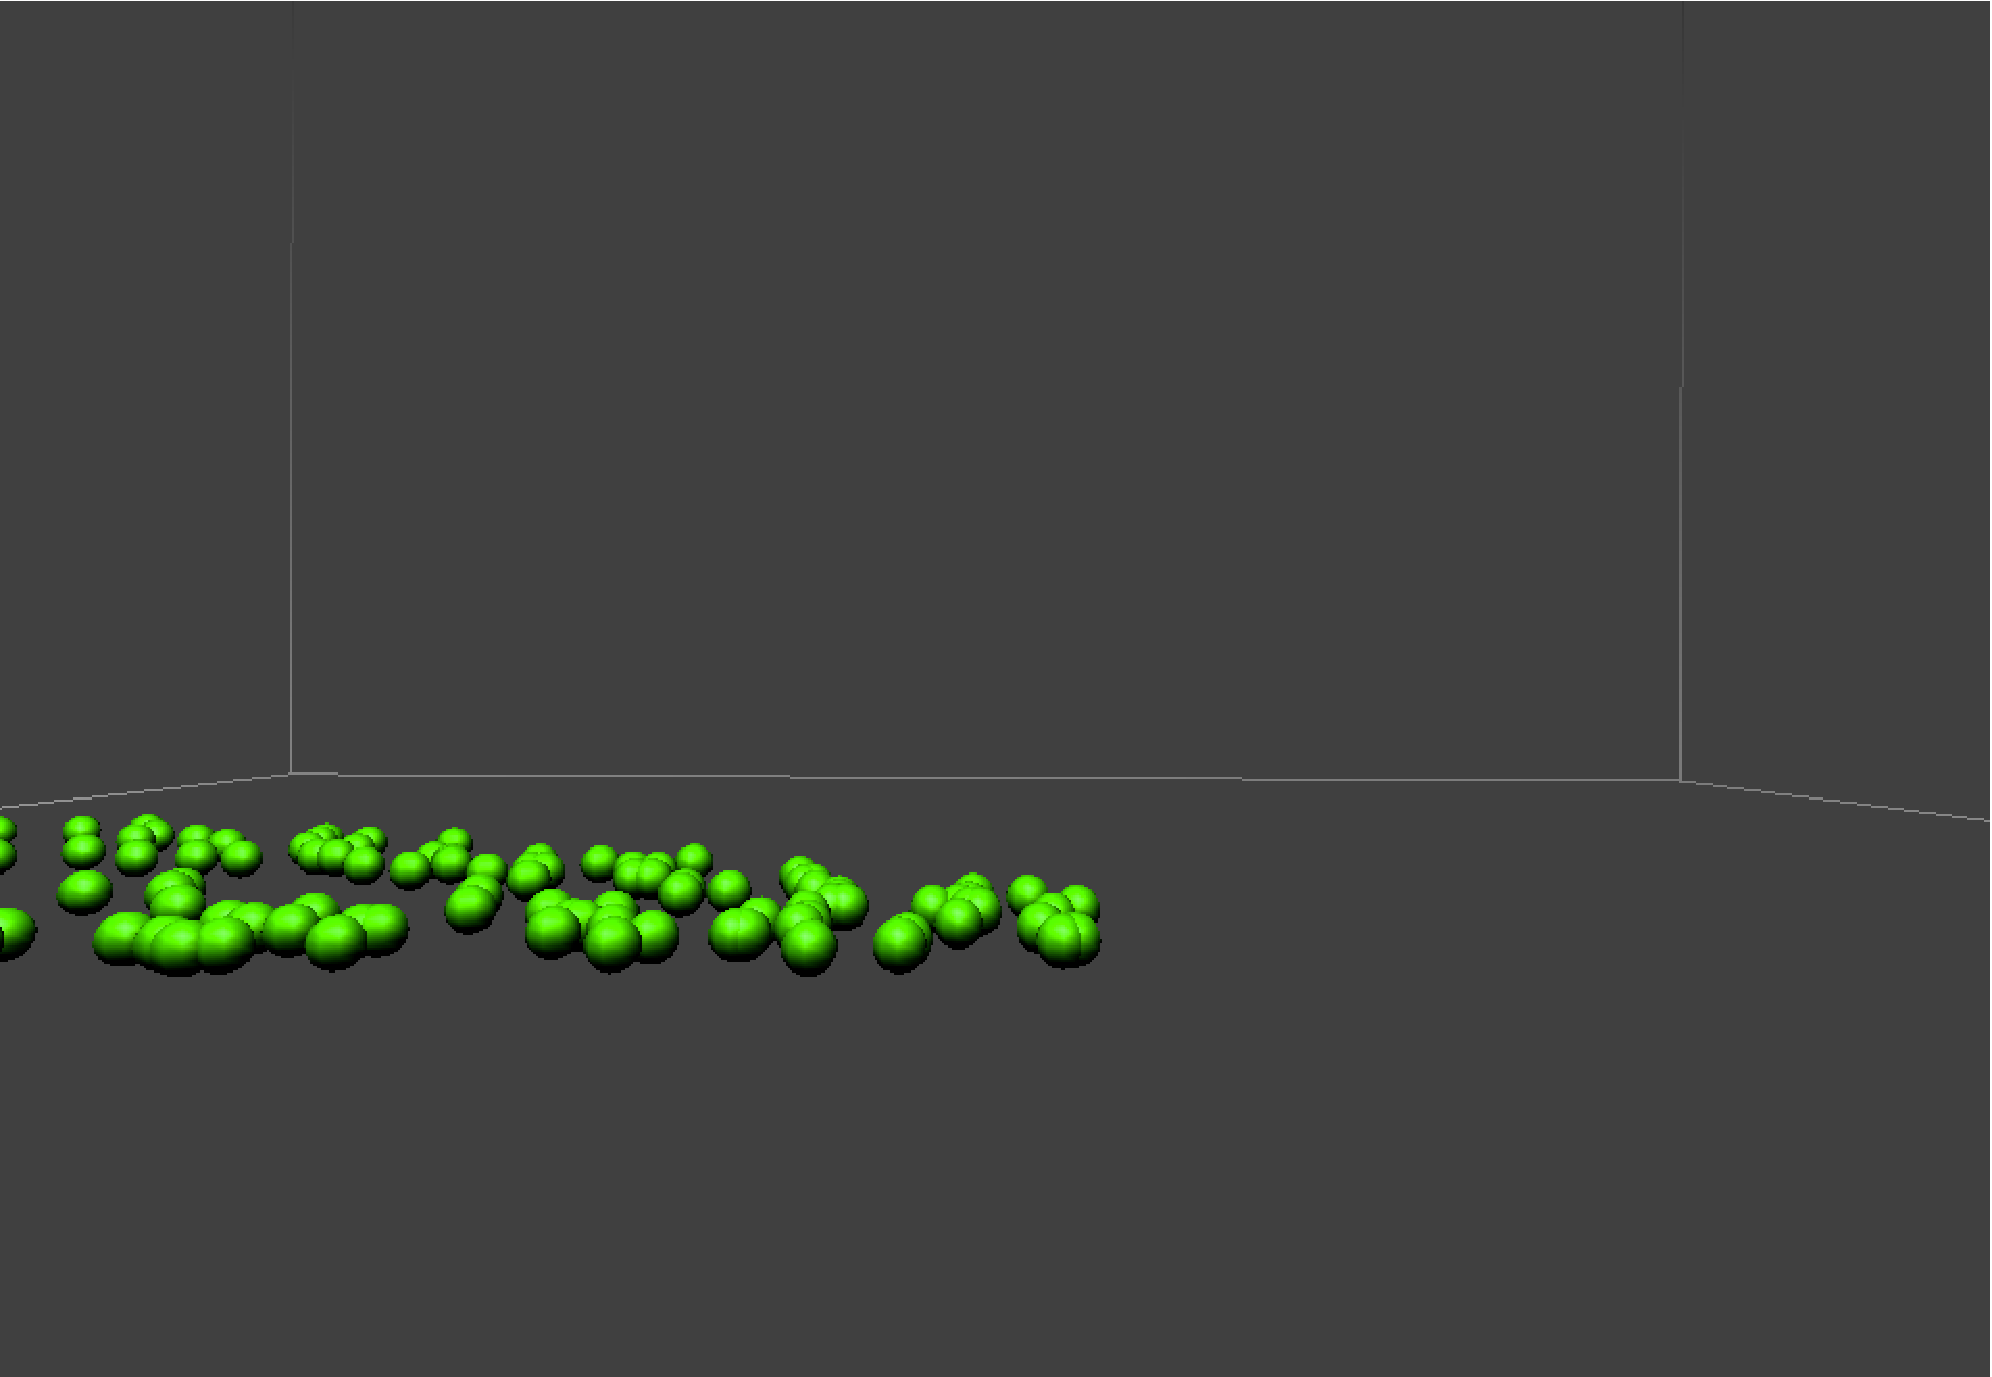
\includegraphics[scale=0.28]{figures/demo_crowds2.pdf} \\
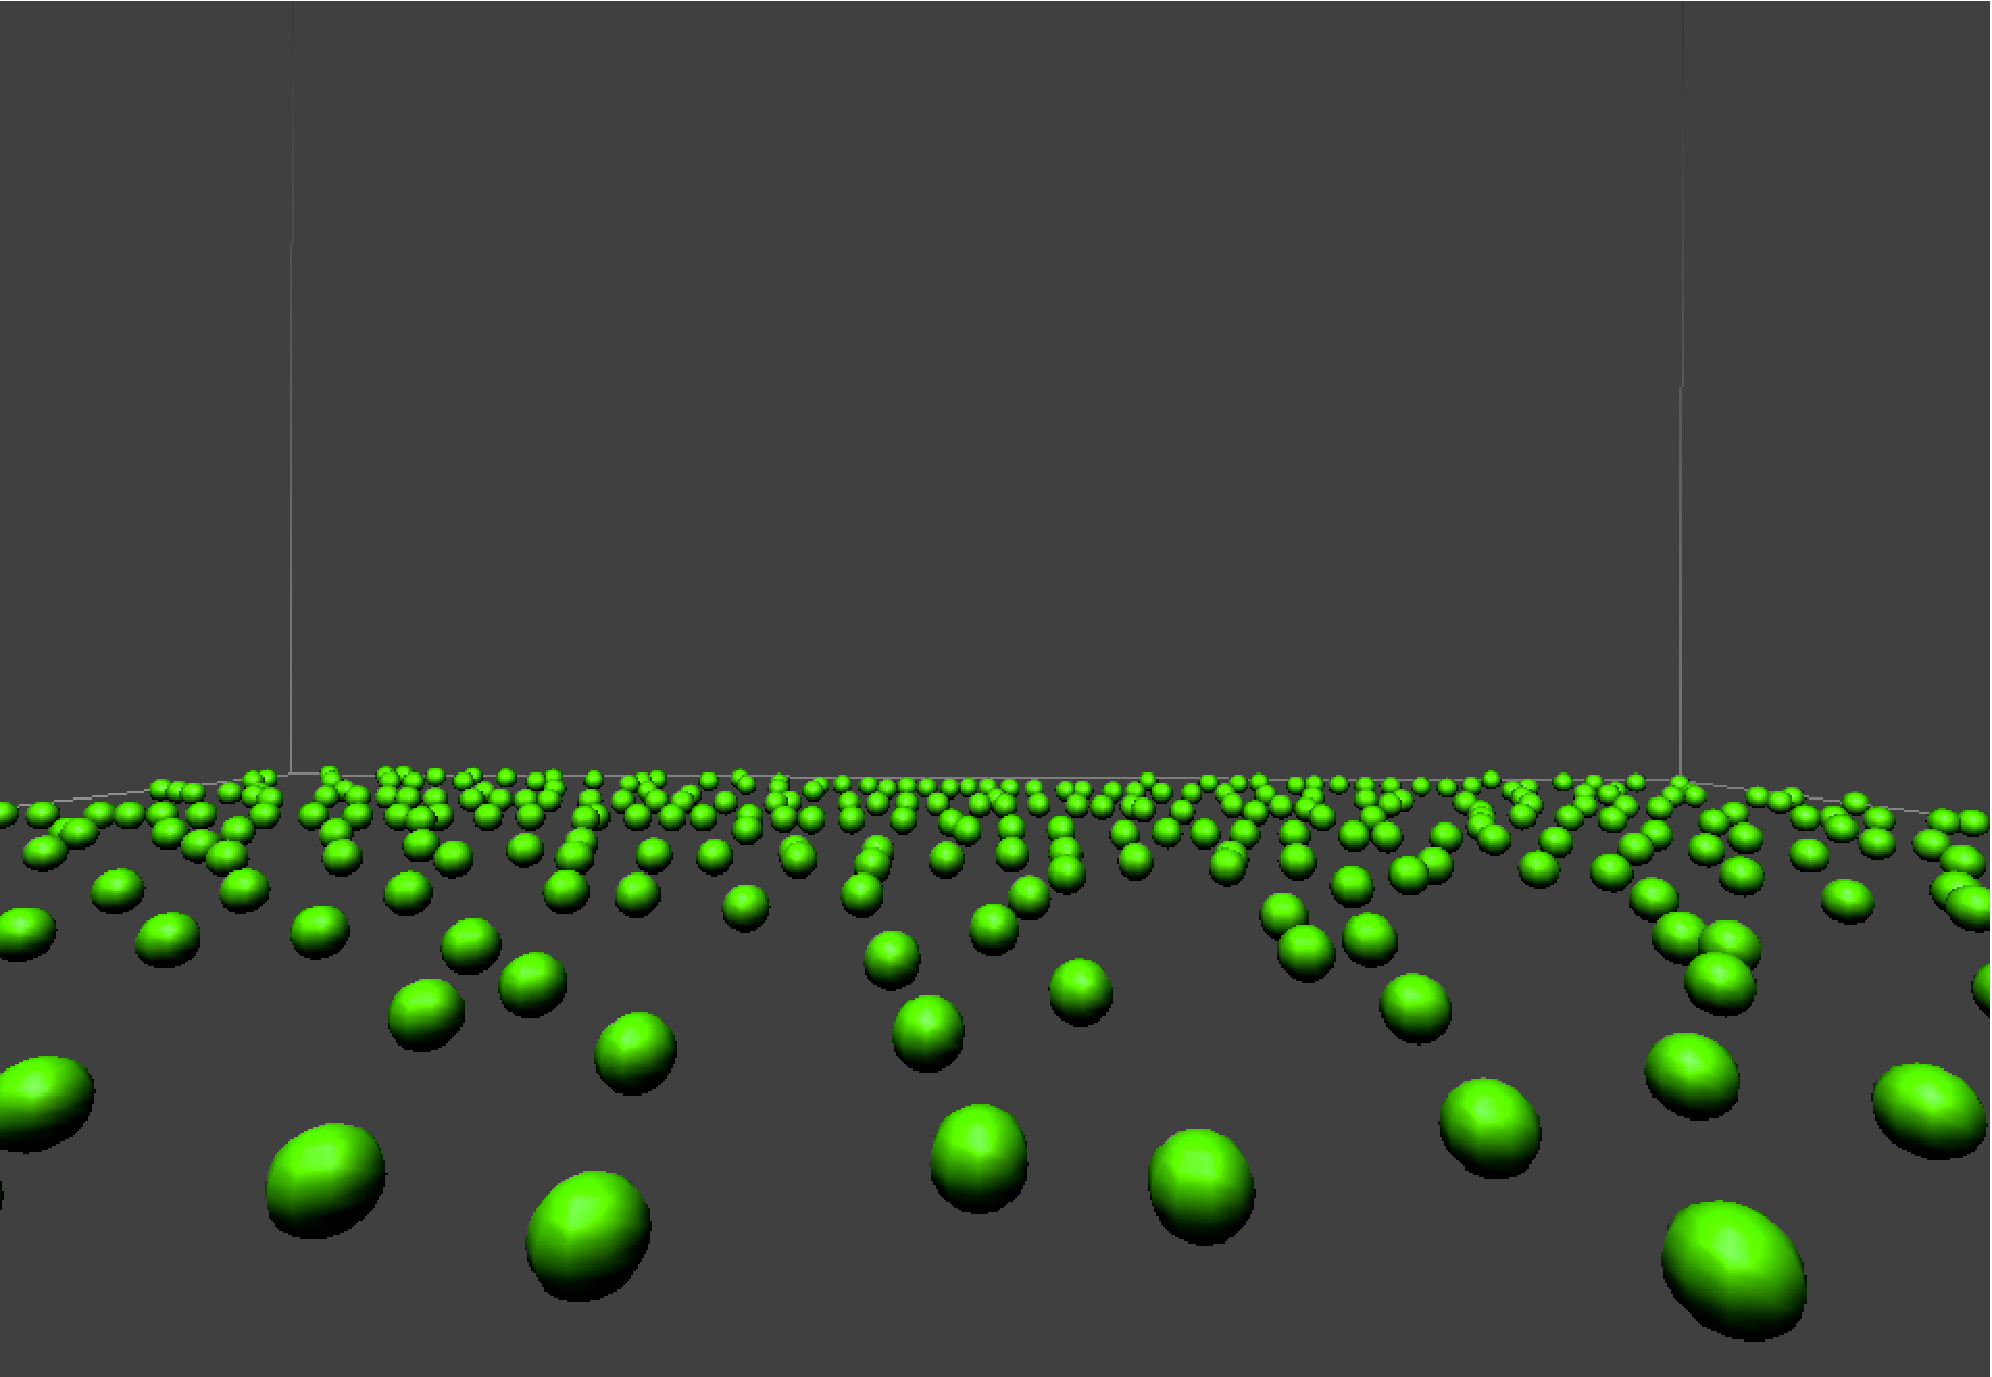
\includegraphics[scale=0.28]{figures/demo_crowds3.pdf}
\end{array}$
\end{center}
\caption{Screenshots of the ``\textit{crowding}'' simulation showing the initial hose, the boids moving, and the boids already spread out throughout the world domain.}
\label{crowd_shots}
\end{figure}



